\documentclass[10pt]{beamer}
\usepackage{makecell}
\usepackage{amssymb,amsmath}
\usepackage{graphicx}
\usepackage{url}
\usepackage{color}
\usepackage{pagenote}[continuous,page]
\usepackage{relsize}		% For \smaller
\usepackage{url}			% For \url
\usepackage{epstopdf}	% Included EPS files automatically converted to PDF to include with pdflatex

%For MindMaps
% \usepackage{tikz}%
% \usetikzlibrary{mindmap,trees,arrows}%

%%% Color Definitions %%%%%%%%%%%%%%%%%%%%%%%%%%%%%%%%%%%%%%%%%%%%%%%%%%%%%%%%%
%\definecolor{bordercol}{RGB}{40,40,40}
%\definecolor{headercol1}{RGB}{186,215,230}
%\definecolor{headercol2}{RGB}{80,80,80}
%\definecolor{headerfontcol}{RGB}{0,0,0}
%\definecolor{boxcolor}{RGB}{186,215,230}

%%% Save space in lists. Use this after the opening of the list %%%%%%%%%%%%%%%%
%\newcommand{\compresslist}{
%	\setlength{\itemsep}{1pt}
%	\setlength{\parskip}{0pt}
%	\setlength{\parsep}{0pt}
%}

%\setbeameroption{show notes on top}

% You should run 'pdflatex' TWICE, because of TOC issues.

% Rename this file.  A common temptation for first-time slide makers
% is to name it something like ``my_talk.tex'' or
% ``john_doe_talk.tex'' or even ``discrete_math_seminar_talk.tex''.
% You really won't like any of these titles the second time you give a
% talk.  Try naming your tex file something more descriptive, like
% ``riemann_hypothesis_short_proof_talk.tex''.  Even better (in case
% you recycle 99% of a talk, but still want to change a little, and
% retain copies of each), how about
% ``riemann_hypothesis_short_proof_MIT-Colloquium.2000-01-01.tex''?

\mode<presentation>
{
  \usetheme{CambridgeUS}
  \usecolortheme{dolphin}
  \useoutertheme{default}
  \useinnertheme{default}
  \setbeamercovered{invisible} % or whatever (possibly just delete it)
}
\beamertemplatenavigationsymbolsempty

\usepackage[english]{babel}
%\usepackage[latin1]{inputenc}
\usepackage{subfigure}

\usepackage{times}
\usepackage[T1]{fontenc}
\usepackage{CJKutf8}

%% makes the ppagenote command for figure references at the end.
\makepagenote
\renewcommand{\notenumintext}[1]{}
\newcommand{\ppagenote}[1]{\pagenote[Page \insertframenumber]{#1}}

\title[Experiment Design (01CH740)]{Experiment Design for Computer Sciences (01CH740)}
\author[Claus Aranha]{Claus Aranha\\{\footnotesize caranha@cs.tsukuba.ac.jp}}
\institute[U. Tsukuba]{University of Tsukuba, Department of Computer Sciences}



% TODO: this class needs more real examples from real data.


\title[]{Experiment Planning and Design}
\subtitle[]{Lecture 5: Techniques for Hypothesis Testing}
\author[Claus Aranha]{Claus Aranha\\{\footnotesize caranha@cs.tsukuba.ac.jp}}
\institute{Department of Computer Science}
\date{2015-06-02}

\begin{document}

\section{Introduction}
\subsection{Outline}

\begin{frame}
  \maketitle
\end{frame}

\begin{frame}
  \frametitle{Outline}
  \begin{block}{}
    Techniques for hypothesis testing in specific situations
  \end{block}
  \begin{itemize}
  \item Calculation of $\alpha$ and $\beta$
  \item Power of a test, and sample size
  \item Testing Variances and Distributions
  \item Non-parametric testing, Difference testing, and Proportional Testing
  \end{itemize}
\end{frame}

\section{Homework Review}
\subsection{Homework Review}
\begin{frame}
  \frametitle{Homework Review}

  \begin{block}{Describe Your Data}
    \begin{itemize}
    \item Analyze your data (or sample data) using statistical means
    \item Means, Variances, Confidence interval
    \item Draw a simple hypothesis test about your data
    \end{itemize}
  \end{block}
\end{frame}

\begin{frame}
  \frametitle{Best report (R.Y.)}
  {\small
  \begin{block}{}
    Comparison of temperature data for months May and July in ``air quality'' data set.
  \end{block}

  \begin{enumerate}
  \item Simple analysis of the data with mean, var, max and min (maybe SD would be better?)
  \item Drawing plots of the two sets of interest:\\
    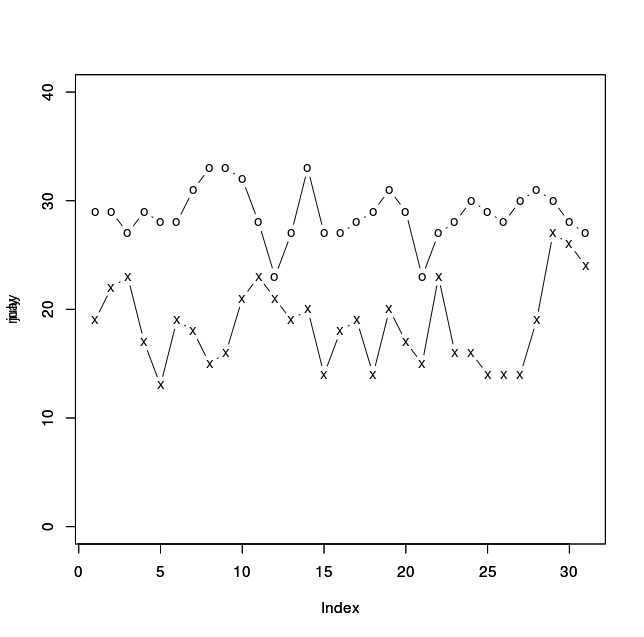
\includegraphics[height=0.4\textheight]{img/yamamoto1}\hspace{1cm}
    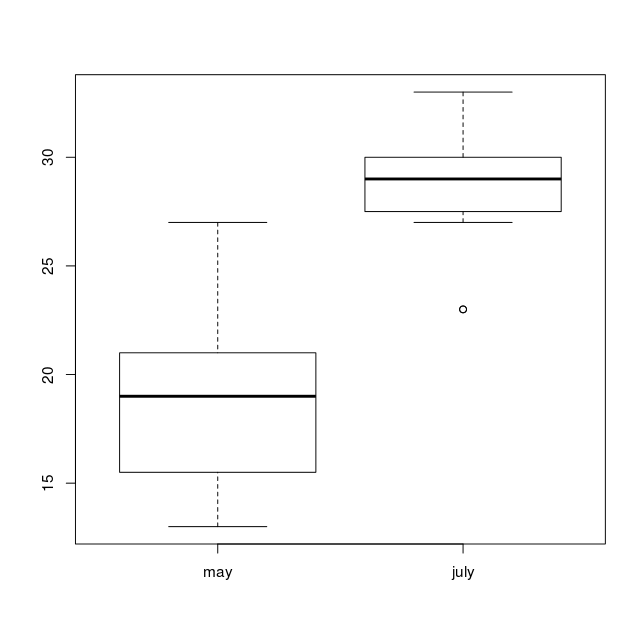
\includegraphics[height=0.4\textheight]{img/yamamoto2}
  \item A difference is observed. To confirm this difference, a hypothesis test is made.
  \end{enumerate}}
\end{frame}

\begin{frame}[fragile,singleslide]
  \frametitle{Best report (R.Y.)}
  {\small
  \begin{block}{}
    Comparison of temperature data for months May and July in ``air quality'' data set.
  \end{block}

  \begin{enumerate}
  \item Kolmogorov-Smirnov test (KS-test) to determine the
    distribution of the data sets (goodness of fit)
\begin{verbatim}
> ks.test(may,"pnorm",mean=mean(may),sd=sd(may))
D = 0.1072, p-value = 0.8683
\end{verbatim}
  \item F-test to compare the variances of the two data sets
\begin{verbatim}
> var.test(may, july)
F = 2.4769, num df = 30, denom df = 30, p-value = 0.01538
\end{verbatim}
  \item Because the variances are different, use Welsh's t-test.
\begin{verbatim}
> t.test(may,july,var.equal=F)
t = -12.66, df = 50.829, p-value < 2.2e-16
\end{verbatim}
  \item Hypothesis test confirms the observation that July is bigger than may.
  \end{enumerate}}
\end{frame}

\begin{frame}
  \frametitle{Common Mistakes: Lack of testing} 
   {\small 

     Many of you calculated mean, variance, and plots for two or more
     variables. Based on these values, you reported some trend.

     \begin{block}{}
       The figure shows that car 1 is faster than car 2
     \end{block}
     
     \begin{itemize}
     \item Eye observation is good for guessing facts about the data,
       but is not good enough for confirming these facts.
     \item Comparing CI intervals is a little better, but not
       completely -- it describes data, but does not infer
       relationships.
     \item Ideally, you should perform \structure{hypothesis tests} to
       confirm the instincts that you obtained from pure observation.
     \end{itemize}

     \alert{Remember that humans suffer from confirmation bias!}

   }
\end{frame}

\begin{frame}
  \frametitle{Common Mistakes: Lack of testing}
  {\small
    
    \begin{center}
      {\renewcommand{\arraystretch}{2}
      \begin{tabular}{|c|c|}
        \hline
        1. Observe Trend in Data & 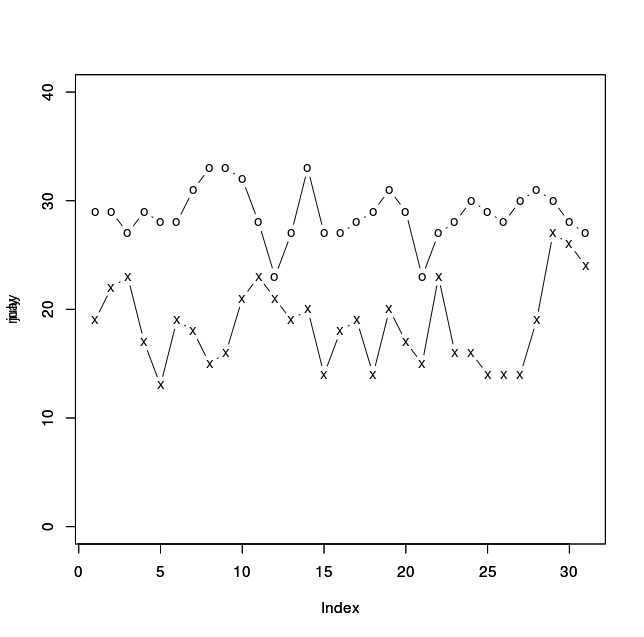
\includegraphics[height=0.2\textheight]{img/yamamoto1}\\
        \hline
        2. Formulate Hypothesis & \makecell{{\bf Null Hypothesis}: means are equal.\\{\bf Alternate Hypothesis}: means are different}\\
        \hline
        3. Hypothesis Testing &  t.test(may,july,var.equal=F)\\
        \hline
        4. Make a decision & ``We can reject the null hypothesis''\\
        \hline
      \end{tabular}}
      
      \bigskip
      
      \begin{alertblock}{}
        Remember, though: this cannot be purely mechanical! You need
        to be conscious about what each step means for your
        experiment!
      \end{alertblock}
    \end{center}    
    }
\end{frame}

\begin{frame}
  \frametitle{Bad Mistake: Parroting}
  \begin{columns}[T]
    \column{0.2\textwidth}
    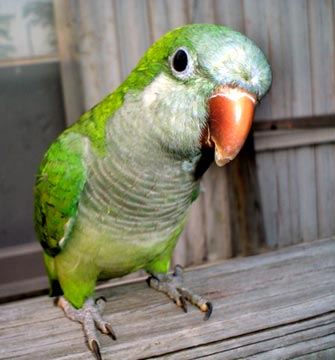
\includegraphics[width=\textwidth]{img/parrot}
    \column{0.8\textwidth}
    \begin{block}{}
      The professor wants tests, so I will do... tests... *squawk!*
    \end{block}
    
    \smallskip

    > t.test(car)\\
    \emph{...any result...}\\

    \smallskip

    ``The test showed that the average of car is bigger than the average of bycicle!''
  \end{columns}

  \bigskip

  
  {\small
    \begin{itemize}
    \item First: \structure{Tests} only exist in the context of
      \structure{questions}.\\ \alert{It makes no sense to make a test
        if you do not decide what are you testing beforehand}
    \item Second: t.test without parameters test
      the sample against the null hypothesis ``mean is equal to 0'', and
      the alternative hypothesis ``mean is different than zero''
    \item \alert{Important:} If you do not understand a concept --
      please ask questions! You will not learn if you don't ask
      questions.
    \end{itemize}
    }

  
  \vfill
  
  \hrule {\tiny Image taken from
    \url{http://www.eurosavant.com/2010/02/01/is-that-a-parrot-in-your-pocket-or/}}
\end{frame}

\begin{frame}
  \frametitle{Homework: Conclusions}
  \begin{itemize}
    \item Each of you should have received a \structure{grade} and
      some \structure{comments} on Manaba.
      \bigskip

    \item These grades \alert{will not} influence your final grade
      \bigskip

    \item However, these grades should give you a good idea of how I
      will evaluate the final report.
      \bigskip

  \end{itemize}

  \begin{center}
    
\includegraphics[width=0.8\textwidth]{img/phd}
  \end{center}

  \hrule
      {\tiny Image from PhdComics: \url{http://www.phdcomics.com/comics/archive.php?comicid=974}}
\end{frame}

\section{Tying up Hypothesis Testing}
\subsection{Review}
\begin{frame}
  \frametitle{Review of Last Lecture (1)}
  \begin{block}{Experimental Hypothesis}
    During an experiment, we \structure{observe} a characteristic of
    the data. This allows us to formulate a \structure{hypothesis},
    which can be tested to confirm or refute our observation.
  \end{block}

  For example:

  \begin{itemize}
  \item The average weight of the part produced by this machine is 500g
  \item The air polution in this city is 15ppm;
  \item Method A is faster than method B by 10\%;
  \item Participants in a survey like chocolate more than vanilla
  \item This method has best performance when $\rho = 60$;
  \end{itemize}
\end{frame}

\begin{frame}
  \frametitle{Review of Last Lecture (2)} 

  {\small After we decide what is the \structure{effect} that we are
  \structure{measuring}, we have to formulate a \structure{null
    hypothesis} and an \structure{alternate hypothesis} that describe
  our observation.}

  \begin{exampleblock}{Null Hypothesis}
    \small
    The null hypothesis usually states that \structure{there is no
      relationship between the factors we are studying}. Or
    \structure{any differences that we see are not significant}. 
    \medskip

    The Null hypothesis indicates the ausence of an effect.
  \end{exampleblock}

  \begin{exampleblock}{Alternate hypothesis}
    \small
    The Alternative hypothesis indicates the presence of \structure{an
      effect}.
  \end{exampleblock}

  \bigskip

  {\small We cannot ``prove'' the alternate hypothesis. We can show that it is
  \structure{much more likely} than the null hypothesis (which we call
  ``rejecting the null hypothesis''.}
\end{frame}

\begin{frame}
  \frametitle{Examples of Null Hypothesis}
  {\small
  {\renewcommand{\arraystretch}{2}
  \begin{tabular}{ll}
  Factors & Null Hypothesis\\ 
  \hline   
  Methods (A,B), Speed & \parbox[t]{0.5\textwidth}{The speed of the
    process is independent of the method}\\  
  Air Pollution, Cities in region & \parbox[t]{0.5\textwidth}{The air
    pollution in all cities in this region is the same}\\
  Parameter $\rho$, Efficiency& \parbox[t]{0.5\textwidth}{The method
    has the same efficiency for any value of $\rho$}\\ Individual
  Machine, Part Weight& \parbox[t]{0.5\textwidth}{The average
      weight of the parts produced by all machines is the same}\\
  \hline
  \end{tabular}}}

  \bigskip

  Of course, determining the right hypothesis is a bit of an art. It
  requires practice, knowledge of your own research, and reflection.

\end{frame}

\begin{frame}
  \frametitle{Review of Last Lecture (3)}

  \begin{block}{Testing the hypothesis}
    After we define the hypothesis, we will have enough information to
    run a statistical test. The statistical test will usually get us:
  \end{block}

  \begin{itemize}
  \item Estimated value for the parameter of interest;
  \item Confidence interval for the parameter of interest;
  \item \structure{p-value} for the alternate hypothesis;
  \item Other information;
  \end{itemize}

  \bigskip
  \begin{block}{P-value}
    Probability that, given the null hypothesis, the experiment 
    result would be that much, or higher.

    \medskip

    If the \structure{p-value} is low enough (depends on the problem,
    0.05 is standard), you can \structure{reject the null hypothesis}
  \end{block}
\end{frame}

\begin{frame}
  \frametitle{Review of Last Lecture (4)}
  \vspace{.3cm}
  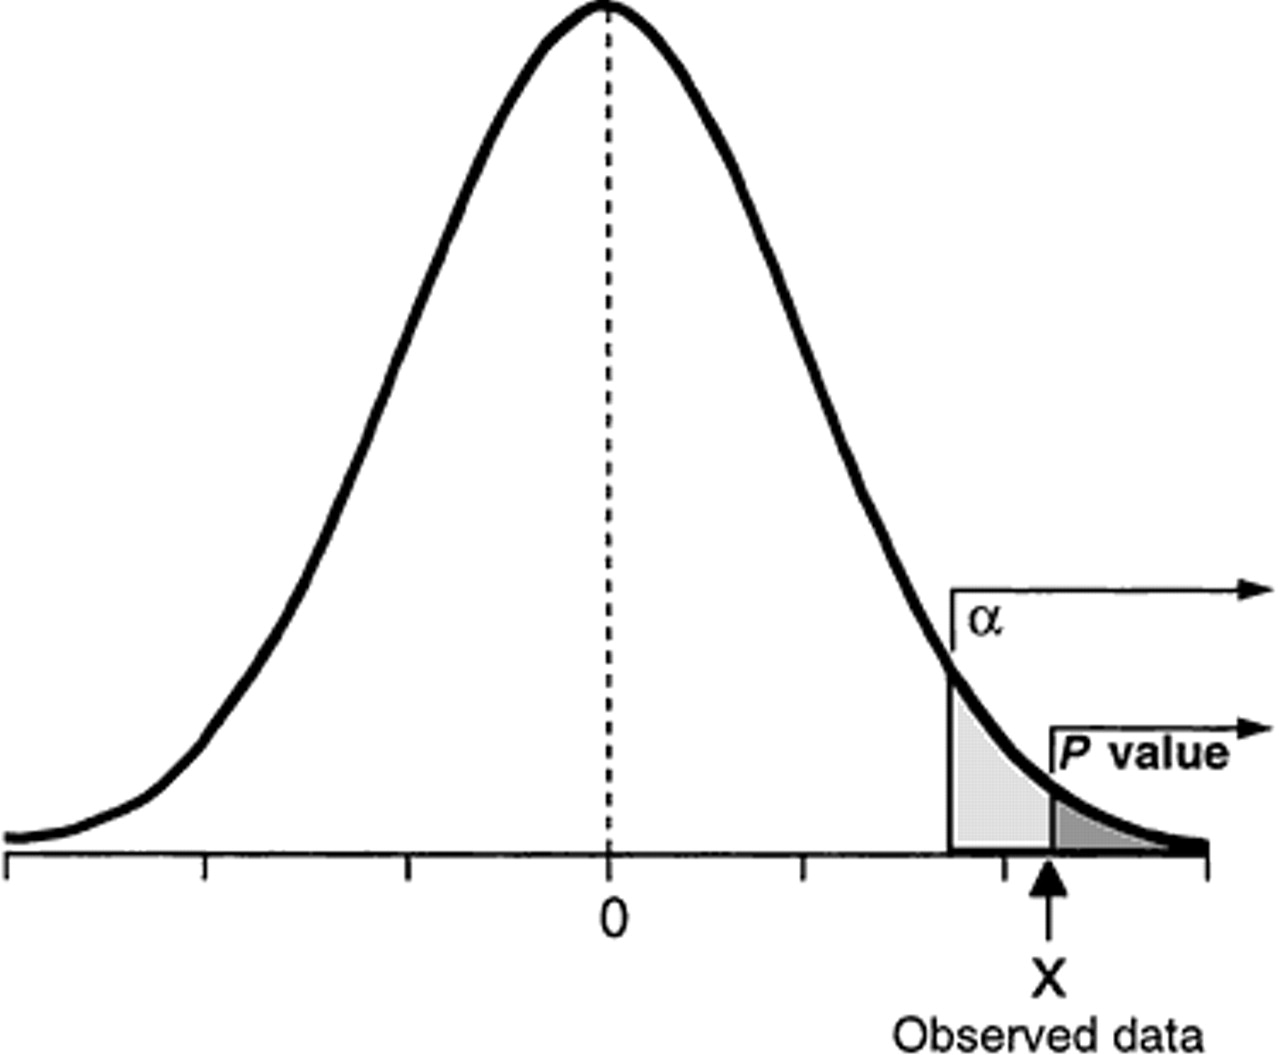
\includegraphics[width=.5\textwidth]{img/pvalue}

  \bigskip

  \structure{$\alpha$ value}: Parameter of the testing procedure that
  decides the desired accuracy.

  \smallskip

  \structure{p-value}: Probability that, given the null hypothesis, the
  experiment result would be that much or higher.

  \hrule
  \hfill\tiny{Image from Steven N. Goodman, \emph{``Towards Evidence Based Medical Statistics''}}
\end{frame}

\begin{frame}
  \frametitle{Example of Hypothesis Testing}
  \begin{block}{Algorithm Analysis}
    {\smaller
    A new algorithm (GA) is used for modeling. We hope that this
    algorithm produces better models than the (RI) algorithm, as
    measured by their log-likelihood.
    \begin{itemize}
      
    \item \structure{Null Hypothesis:} Log likelihood of the model is
      independent of the method used (for methods GA and RI)
    \item \structure{Alternate Hypothesis:} Log likelihood of models
      generated by GA are higher than the value generated by RI
      models.
    \end{itemize}}
  \end{block}
  \begin{center}
  \small{
    \begin{tabular}{|c|c|c|c|}
      \hline
          {Scenario} & \multicolumn{3}{|c|}{Log Likelihood}\\
          & RI & GA & p-value\\
          \hline
          2005 & -2263.4      &-2253.2 (16.5) & 0.01 \\%& 0.38 & 0.24 & 0.24 (0.04) & 0.78\\
          2006 & -2252.28     &-2234.72 (14) & 0.01 \\%& 0.36 & 0.10 & 0.18 (0.01) & 0.01 \\
          2007 & -2113.84      &-2108.95 (11.1) & 0.03 \\%& 0.36 & 0.15 & 0.19 (0.02) &  0.01 \\
          2008 &-2110.79      &-2096.75 (11.8) & 0.01 \\%& 0.39 & 0.16 & 0.22 (0.03) & 0.01 \\
          2009 &-2487.88      &-2482.88 (10.3) & 0.02 \\%& 0.36 & 0.09 & 0.14 (0.01) & 0.01 \\
          2010 &-2132.11      &-2099.13 (16.3) & 0.01 \\%& 0.39 & 0.14 & 0.28 (0.03) & 0.01 \\
          2011 &-20083.09    &-19983.73 (144.4) & 0.01 \\%& 0.35 & 0.07 & 0.08 (0.02) & 0.14\\
          2012 &-3225.39     &-4435.34 (248) & 1.00 \\%& 0.48 & 0.80 & 0.77 (0.01) & 1.00 \\
          \hline
    \end{tabular}
  }
  \end{center}
\end{frame}

\begin{frame}
  \begin{center}
    Can we start with new material?
  \end{center}
\end{frame}

\subsection{Power and Effects of interest}

\begin{frame}
  \frametitle{Types of Errors}

  In the last class, we defined two types of errors: 
  \begin{itemize}
  \item \alert{Type I errors}: rejecting the null hypothesis when it should
    not be rejected (false positive)
  \item \structure{Type II errors}: not rejecting the null hypothesis when it
    should be rejected (false negative)
  \end{itemize}
  
  \bigskip

  \begin{block}{}
    A type I error depends only on the significance level $\alpha$, which
    is a parameter we control;

    \medskip

    The probability of a type II error is defined by the \emph{power}
    of a test, defined by $\beta$.
  \end{block}
\end{frame}

\begin{frame}
  \frametitle{How to control for type II error?}
  The power of a test is defined by 4 factors
  \begin{enumerate}
  \item Actual size of the difference
  \item Variability of the observations
  \item Significance level
  \item Sample size
  \end{enumerate}
  
  \begin{block}{Minimally interesting effect}
    One way to estimate a lower bound for the power of a test is by
    defining a \emph{minimally interesting effect} $\delta*$

    \bigskip

    It is essential to have a good understanding of the problem in
    order to define this value.    
  \end{block}

\end{frame}

\begin{frame}[singleslide,fragile]
  \frametitle{Example of power calculation}

{\small Suppose that on the green peas example one is really interested in
detecting deviations from the nominal value greater than $1\%$, i.e.,
$\delta^* = 0.01*500 = 5g$. The researcher defines that, for this
minimally interesting effect, a tes t power of $0.85$ is desired. The
test will again be performed with $\alpha = 0.01$.

\smallskip

The same sample of $n=10$ packs is used. The estimated standard
deviation for this sample is $s=6.97g$. From this data, we can compute
the power of this test as:}
{\small
\begin{verbatim}
> s<-sd(sample)
> power.t.test(n=10, delta=5, sd=s, sig.level=0.01, 
+        type = "one.sample", alternative = "one.sided")
\end{verbatim}

\begin{verbatim}
One-sample t test power calculation 
n = 10
delta = 5
sd = 6.970382
sig.level = 0.01
power = 0.3474724
alternative = one.sided
\end{verbatim}}
\end{frame}

\begin{frame}[singleframe,fragile]
  \frametitle{Example of sample size calculation}
  What is the smallest sample size needed to obtain the desired power of $0.85$?

  \medskip
\begin{verbatim}
> power.t.test(power=0.85, delta=5, sd=s, sig.level=0.01,
  type = "one.sample", alternative = "one.sided")

One-sample t test power calculation 
n = 24.76091
delta = 5
sd = 6.970382
sig.level = 0.01
power = 0.85
alternative = one.sided
\end{verbatim}

\bigskip

We need at least 25 observations to detect a $-5g\ (1\%)$ or larger
deviation on the mean weight of the green peas packages with a power
level of $0.85$.
\end{frame}

\subsection{Testing Assumptions} % Variance, Distribution

\begin{frame}
  \frametitle{Hypothesis Testing Types}
  
  \begin{itemize}
  \item Last week we saw a simple example of statistical testing
    calculation (t-test)
  \item The t-test makes many assumptions about the data (normal
    distribution, known variance, etc)
  \item To break these assumptions, we need slightly different
    statistical methods.
  \end{itemize}
  \vfill

  \small{\hfill Reference: Peter Dalgaard, ``Introductory Statistics
    wih R'' (Chapters 5,7,8)}
\end{frame}

\begin{frame}[fragile,simpleframe]
  \frametitle{One Sample t-test}
  \begin{itemize}
  \item Assumes that the data comes from the \structure{normal}
    distribution $N(\mu,\sigma)$;
  \item We estimate $\mu$ and $\sigma$ from the mean and standard
    deviation of the sample;
  \item We compare the $\mu$ of the sample with a single value
    $\mu_0$. This is the null hypothesis.
  \item The $t$ statistic is given by:
    \begin{equation*}
      t = \frac{\bar{x} - \mu_0}{\sigma/\sqrt{n}}
    \end{equation*}
  \item The $t$ value is compared to the critical regions in the
    Normal distribution to define the \emph{p value};
  \end{itemize}
\end{frame}

\begin{frame}[fragile,simpleframe]
  \frametitle{One Sample t-test -- example}
{\small
\begin{verbatim}
> install.packages("ISwR")
> library(ISwR)
> attach(intake); pre
  [1] 5260 5470 5640 6180 6390 6515 6805 7515 7515 8230 8770

> t.test(pre,mu=7725)

        One Sample t-test

data:  pre 
t = -2.8208, df = 10, p-value = 0.01814
alternative hypothesis: true mean is not equal to 7725 
95 percent confidence interval:
 5986.348 7520.925 
sample estimates:
mean of x 
 6753.636
\end{verbatim}
}
\end{frame}

\begin{frame}
  \frametitle{One Sample t-test -- arguments}
  \begin{itemize}
  \item t.test(data,mu=9000,alternative="greater")\\
    Does a one-tailed test ($h_a$ is true mean is greater than $h_0$);
  \item t.test(data,mu=9000,alternative="less")
  \item t.test(data,mu=9000,conf.level=0.99)
    Changes the required confidence level to 99\%;
  \end{itemize}
\end{frame}

\begin{frame}
  \frametitle{Assumptions for the one sample t-test}
  
  The t-test (and the z-test as well) make a few assumptions about the
  nature of the data:

  \bigskip

  \begin{itemize}
  \item The distribution of the population is approximately normal;
  \item Indenpendence of Residuals (abscense of outside factors);
  \item Equal variance (in case of multiple samples, see later);
  \end{itemize}

  \bigskip

  We can test these assumptions in two ways:
  \begin{itemize}
  \item Graphical/Qualitative Tests;
  \item Analytical/Quantitative Tests;
  \end{itemize}
\end{frame}

\begin{frame}[fragile,simpleframe]
  \frametitle{Normality Assumption (1)}
  \begin{block}{}
    The QQ plot is a great tool to verify if your data follows a certain distribution.
\begin{verbatim}
> qqnorm(pre)
> rpois(10,5)
 [1] 10 10  2  5  5  4  7  7  4  4
> qqnorm(rpois(10,5))
\end{verbatim}
  \end{block}
  \begin{center}
    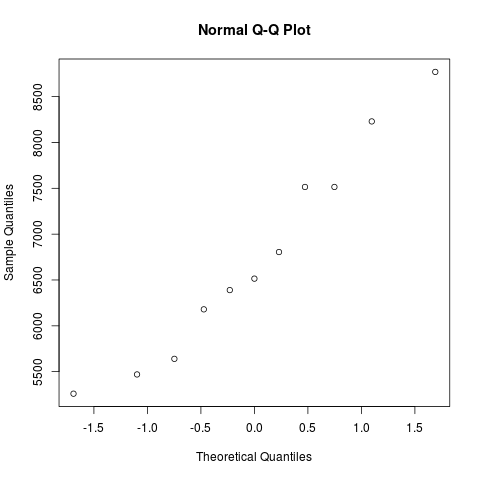
\includegraphics[width=0.4\textwidth]{img/qqplot_intake}
    \hfill
    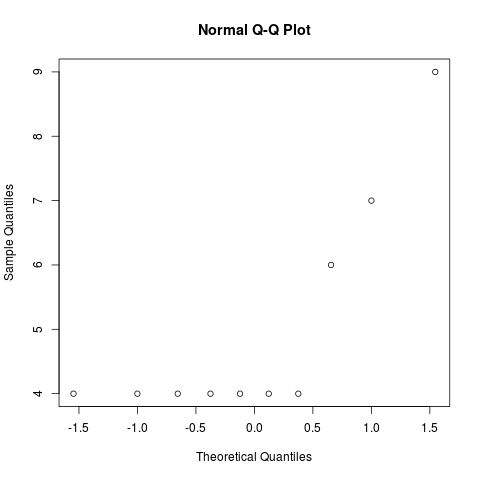
\includegraphics[width=0.4\textwidth]{img/qqplot_poisson}
  \end{center}
\end{frame}

\begin{frame}[singleframe,fragile]
  \frametitle{Normality Assumption (2)}

  There is a large number of statistical methods for normality
  testing. We saw previously the NK test. Another quite used test is
  the Lilliefors test.

  Even thought the Lilliefors test is possibly the most widely used
  for normality testing, the Shapiro-Wilk test tends to be more
  sensitive and has some other interesting properties, so we will be
  using it throughout the course. 
\begin{verbatim}
> shapiro.test(sample)
    
Shapiro-Wilk normality test
data:  sample
W = 0.8809, p-value = 0.1335
\end{verbatim}
\end{frame}

\begin{frame}
  \frametitle{Summary of part I}
  \begin{itemize}
  \item Look at your data, and formulate the null and alternate hypothesis;


  \item The t.test is normally used for comparison of a single sample
    against pontual values;


  \item The t.test assumes that 
    \begin{itemize}
    \item \structure{the samples are independent},
    \item \structure{the population is normally distributed},
    \item \structure{multiple samples have the same variance}
    \end{itemize}

  \item You need to test for each of these assumptions, or risk
    getting imprecise, or wrong, results.
  \end{itemize}

  \bigskip

  Any questions?

\end{frame}

\section{Specialist Tests}
\subsection{Non-parametric Testing}

\begin{frame}
  \frametitle{Non-normal distributions}

  We said that the t-test \structure{assumes that the distribution is
    normal}. So what do we do if we find out that our distribution is
  non-normal?

  \bigskip

  Actually, most cases of non-normality can be solved with judicial
  application of the \structure{Central Limit Theorem}. Do you still
  remember it?

  \bigskip
  
  Still, for some cases, that is not enough. This is specially true
  for data that has \structure{no clear scale}. So what do we do?
  
  \bigskip

  \begin{center}
    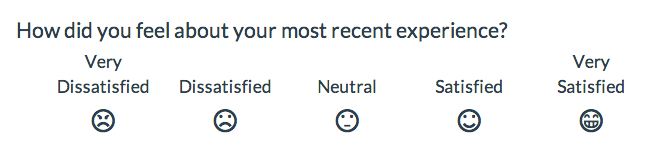
\includegraphics[width=.8\textwidth]{img/likert_scale}
  \end{center}
\end{frame}

\begin{frame}
  \frametitle{Wilcoxon Signed-Rank Test (1)}
  
  \begin{block}{Non-parametric Tests}
    Non-parametric tests ignore the absolute differences between data,
    and consider relative differences;

    For example, the Wilcoxon test calculates the ranks of each sample
    (best, second, third...). The statistical test is made on these
    rank values.
  \end{block}
\end{frame}

\begin{frame}
  \frametitle{Wilcoxon Signed-Rank Test (2)}

    Consider the following data. We want to compare this data against
    a $h_0$ of 7720.

    \bigskip

    \begin{columns}
      \column{.5\textwidth}
      \begin{tabular}{|c|c|c|}
        \hline
        Sample & Difference & Rank\\
        \hline
        5260 & -2460 & -8\\
        5470 & -2250 & -7\\
        5640 & -2080 & -6\\
        6180 & -1540 & -5\\
        6390 & -1330 & -4\\
        6515 & -1205 & -3\\
        6805 & -915 & -2\\
        7515 & -205 & -0.5\\
        7515 & -205 & -0.5\\
        8230 & 510 & 1.0\\
        8770 & 1050 & 2.0\\
        \hline
      \end{tabular}
      \column{.5\textwidth}
      \begin{itemize}
      \item The ranks are the values of each observation against $h_0$.

        \bigskip

      \item Two observations with the same value share the same rank.
      \end{itemize}
    \end{columns}
\end{frame}

\begin{frame}[fragile,simpleframe]
  \frametitle{Wilcox test example:}
{\small
\begin{verbatim}
> install.packages("ISwR")
> library(ISwR)
> attach(intake); pre
[1] 5260 5470 5640 6180 6390 6515 6805 7515 7515 8230 8770

> wilcox.test(pre, mu=7725)

    Wilcoxon signed rank test with continuity correction

data:  pre 
V = 8, p-value = 0.0293
alternative hypothesis: true location is not equal to 7725 

Warning message:
In wilcox.test.default(pre, mu = 7725) :
  cannot compute exact p-value with ties
\end{verbatim}
}
\end{frame}

\subsection{Difference Testing}

%% TODO: Replace with text from Felipe Campelo
%% https://github.com/fcampelo/Design-and-Analysis-of-Experiments/blob/master/06-SimpleComparisons/Chapter06.pdf
\begin{frame}
  \frametitle{Two sample tests}
  \begin{block}{}
    We want to compare two samples coming from different experiments or treatments.
  \end{block}
  \begin{itemize}
  \item The mathematics behind two-sample statistical testing is
    similar to that of the one-sample test.
    \begin{equation*}
      t = \frac{\bar{\mu_1} - \bar{\mu_2}}{SEDM}
    \end{equation*}
  \item The two-sample tests may be done with the assumption of equal
    variance, or without it. R by default assumes different variances;
  \item The wilcox non-parametric test for two samples is treated in a
    similar manner;
  \end{itemize}
\end{frame}

\begin{frame}[fragile,singleframe]
  \frametitle{Two sample test -- Examples (1)}
\begin{verbatim}
> install.packages("ISwR")
> library(ISwR)
> attach(energy)
> energy
   expend stature
1    9.21   obese
2    7.53    lean
3    7.48    lean
(...)
20   7.58    lean
21   9.19   obese
22   8.11    lean
\end{verbatim}
\end{frame}

\begin{frame}[fragile,singleframe]
  \frametitle{Two sample test -- Examples (2)}
\begin{verbatim}
> t.test(expend~stature)
                                                                                                           
        Welch Two Sample t-test                                                                            
                                                                                                           
data:  expend by stature                                                                                   
t = -3.8555, df = 15.919, p-value = 0.001411                                                               
alternative hypothesis: true difference in means is not
                        equal to 0                                         
95 percent confidence interval:                                                                            
 -3.459167 -1.004081                                                                                       
sample estimates:                                                                                          
 mean in group lean mean in group obese                                                                    
           8.066154           10.297778

\end{verbatim}
\begin{block}{}
\small{Remember: expend~stature indicates that column ``expend'' is explained by column ``stature''}
\end{block}
\end{frame}

\begin{frame}[fragile,singleframe]
  \frametitle{Two sample test -- Examples (3)}
  {\small
\begin{verbatim}

> wilcox.test(expend~stature)                                                                              
                                                                                                           
        Wilcoxon rank sum test with continuity correction                                                  
                                                                                                           
data:  expend by stature                                                                                   
W = 12, p-value = 0.002122                                                                                 
alternative hypothesis: true location shift is not equal to 0                                              
                                                                                                           
Warning message:                                                                                           
In wilcox.test.default(x = c(7.53, 7.48, 8.08, 8.09, 10.15, 8.4,  :                                        
  cannot compute exact p-value with ties

\end{verbatim}
}
\end{frame}

%% TODO: Update the section on proportion testing

\subsection{Proportional Testing}
\begin{frame}
  \frametitle{What are proportion tests}
  \begin{block}{}
    In some experiments, the result is not reported as a numerical
    result, or even as levels. Instead, we have only a
    ``success/failure'' measure.
  \end{block}
  \begin{itemize}
  \item TSP-like problems;
  \item Finding Global Optimals;
  \item Prediction Hit Ratios;
  \item etc;
  \end{itemize}
  \begin{block}{}
    In these cases, we want to use \structure{proportion tests}.
  \end{block}
\end{frame}

\begin{frame}
  \frametitle{Single Proportion Test}
  \begin{itemize}
  \item Test is based on a binomial distribution with size $N$ and
    probability $p$;
  \item The test statistic for $p = p_0$, where $x$ is the number of
    successes, becomes:
    \begin{equation*}
      u = \frac{x - Np_0}{\sqrt{Np_0(1-p_0)}}
    \end{equation*}
  \item $u$ is assumed to have a normal distribution with mean 0 and sd 1;
  \end{itemize}
\end{frame}

\begin{frame}[fragile,singleframe]
  \frametitle{Single Proportion Test (Example)} {\small In a survey,
    39 of 215 randomly selected patients in a hospital have asthma. We
    test the hypothesis of ``the proportion of asthmatic people in the
    hospital is 0.15''.
  \begin{block}{}
\begin{verbatim}
> library(ISwR)
> prop.test(39,215,.15)

        1-sample proportions test with 
        continuity correction

data:  39 out of 215, null probability 0.15 
X-squared = 1.425, df = 1, p-value = 0.2326
alternative hypothesis: true p is not equal to 0.15 
95 percent confidence interval:
 0.1335937 0.2408799 
sample estimates:
        p 
0.1813953
\end{verbatim}
  \end{block}
  \alert{Don't confuse the proportion p with the p-value!}
  }
\end{frame}

\begin{frame}
  \frametitle{The End!}

  (There is more next class)
\end{frame}

% How to define a good significance? (One of the chapters say that)

%%%%%%%%%%%%%%%%%%%%%%%%%%%%%%%%%%%%%%%%%%%%%%%%%%%%%%%%%%%%%%%%%%%%%%%%%%%%%%%%

% Overflow

\section{Specific Tests}

\subsection{Paired Tests}
\begin{frame}
  \frametitle{Paired Tests (1)}
  \begin{columns}[c]
    \column{0.3\textwidth}
    
\includegraphics[width=1\textwidth]{img/soccer}
    \column{0.7\textwidth}
    \begin{block}{}
    How would you test the differences between two types of shoes (A and B)?
    \end{block}
    \begin{enumerate}
    \item Give some kids the shoe A, and some kids the shoe B\\ 
      {\small The personality of the kid becomes a factor -- more agressive
      kids may wear the shoe faster?}
    \item Give each kid one of each shoe: Left shoe A, right shoe B (or random)\\
      {\small In this way each kid will use both shoes equally.}
    \end{enumerate}
    \begin{block}{}
      Can we use this information (same kid used both shoes) to
      improve our statistical testing?
    \end{block}
    \vfill

    \hfill{\tiny Image from http://leagueathletics.com/}
  \end{columns}
\end{frame}

\begin{frame}
  \frametitle{Paired Tests (2)}
  \begin{block}{Interface Testing}
    Imagine you are comparing two HCI technologies using a survey. You
    ask each surveyed person to compare two systems using a score.
  \end{block}
  \bigskip

  \begin{itemize}
  \item Scores given by the same person should show the same biases;
  \item Thus, you want to compare the scores described by the same voters;
  \item \alert{Important!} Don't forget to change the order of voting!
  \end{itemize}
\end{frame}

\begin{frame}[fragile,singleframe]
  \frametitle{Paired T-Test}
  \begin{itemize}
  \item The Paired T-test is based on the idea of calculating the
    difference between the samples. 
  \item This difference is then treated as
    a one-sample test.
  \end{itemize}
  \begin{block}{}
{\small
\begin{verbatim}
> attach(intake)
> pre; post; post-pre
 [1] 5260 5470 5640 6180 6390 6515 6805 7515 7515 8230 8770
 [1] 3910 4220 3885 5160 5645 4680 5265 5975 6790 6900 7335
 [1] -1350 -1250 -1755 -1020  -745 -1835 -1540 -1540  -725 -1330 -1435
\end{verbatim}}
\end{block}
\end{frame}

\begin{frame}[fragile,singleframe]
  \frametitle{Paired T-Test}
  \begin{itemize}
  \item The Paired T-test is based on the idea of calculating the
    difference between the samples. 
  \item This difference is then treated as
    a one-sample test.
  \end{itemize}
  \begin{block}{}
{\small
\begin{verbatim}
> t.test(pre,post,paired=T)

        Paired t-test

data:  pre and post 
t = 11.9414, df = 10, p-value = 3.059e-07
alternative hypothesis: true difference in means 
                             is not equal to 0 
95 percent confidence interval:
 1074.072 1566.838 
sample estimates:
mean of the differences 
               1320.455
\end{verbatim}}
  \end{block}
\end{frame}

\begin{frame}
  \frametitle{Paired T-Test -- Important points 1}
  \begin{itemize}
  \item If your data is paired (there is a correspondence between the
    two samples), you MUST use a paired test for correct results;
  \item Conversely, if your data is NOT paired, you should NOT use a
    paired test;
  \end{itemize}
\end{frame}

\begin{frame}[fragile,singleframe]
  \frametitle{Paired T-Test -- Important points 2}
  \begin{itemize}
  \item The paired t-test \structure{assumes} that the difference between the
    samples is \structure{independent of the level};
  \item This means that higher values do not have a bigger difference
    than lower values;
  \item You can examine this by plotting the difference of the pair
    against the average of the pair;
  \item Even if the differences scales with the level, a
    transformation of the data can be used to fix this problem.
  \end{itemize}
\begin{columns}[c]
  \column{0.6\textwidth}
\begin{verbatim}
plot(pre-post,pre+post/2)
\end{verbatim}
\column{0.4\textwidth}
\hfill 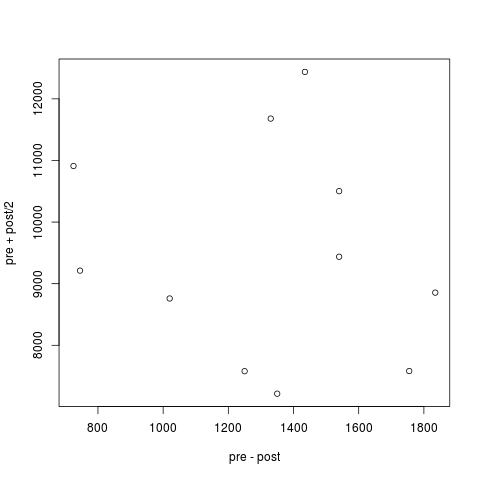
\includegraphics[width=1\textwidth]{img/bland_altman}
\end{columns}
\end{frame}

\begin{frame}[fragile,singleframe]
  \frametitle{Paired Wilcoxon Test}
  \begin{itemize}
  \item The basic idea of the Paired Wilcoxon test is similar to the paired T-test;
  \item The ``rank of the differences'' is calculated; (so the size of the differences has a smaller effect)
  \end{itemize}
  \begin{block}{}
\begin{verbatim}
> wilcox.test(pre,post,paired=T)

        Wilcoxon signed rank test with continuity correction

data:  pre and post 
V = 66, p-value = 0.00384
alternative hypothesis: true location shift is 
                        not equal to 0 

Warning message:
In wilcox.test.default(pre, post, paired = T) :
  cannot compute exact p-value with ties
\end{verbatim}
  \end{block}
\end{frame}

\section{Analysis of Variance} %(Chapter 7)
\subsection{Introduction}
\begin{frame}
  \frametitle{Analysis of Variance}
  \begin{block}{Introduction}
    The Analysis of Variance (ANOVA) is a statistical method for
    testing many samples at the same time.
  \end{block}
  \begin{itemize}
  \item We want to find the best values for 4 parameters in our
    method. Each parameter can be valued between 0.0 and 1.0;
  \item Can we experiment the parameter values two at a time? Why? Why
    not?
  \end{itemize}
\end{frame}

\begin{frame}
  \frametitle{Analysis of Variance (Model)}
  \begin{block}{}
    Let each observation $x_{ij}$ be the $j$-th observation in group
    $i$. We decompose this observation as:
  \end{block}
  \begin{equation*}
    x_{ij} = \bar{x} + (\bar{x_i} - \bar{x}) + (x_{ij} - \bar{x_i})
  \end{equation*}
  \begin{block}{}
    In other words, eath observation is composed by the grand average
    of all samples, plus the deviation of the group, plus the
    (independent) error of the sample.
  \end{block}
\end{frame}

\begin{frame}
  \frametitle{Analysis of Variance (Model)}
  \begin{itemize} 
  \item The Analysis of Variance starts from the assumption that
    the variance of all groups is the same;
  \item If this assumption holds, then we can compare the variance
    difference between groups to test the null hypothesis that
    ``All groups have the same mean'';
  \end{itemize}
  \begin{block}{}
    Although it is called Analysis of Variance, and the main
    calculations are based on the variance of the groups, the final
    goal is a hypothesis centered on the means of the groups.
  \end{block}
\end{frame}

\begin{frame}[fragile,singleframe]
  \frametitle{Analysis of Variance (Example -- 1)}
{\small
  \begin{block}{}
\begin{verbatim}
> attach(red.cell.folate)
> summary(red.cell.folate)
folate          ventilation
Min.   :206.0   N2O+O2,24h:8   
1st Qu.:249.5   N2O+O2,op :9   
Median :274.0   O2,24h    :5   
Mean   :283.2                  
3rd Qu.:305.5                  
Max.   :392.0
\end{verbatim}
  \end{block}}

The red cell folate data set has three different categories: N20+02 24h, op, and O2 24h;

\end{frame}

\begin{frame}[fragile,singleframe]
  \frametitle{Analysis of Variance (Example -- 2)}
{\small
  \begin{block}{}
\begin{verbatim}
> anova(lm(folate~ventilation))
Analysis of Variance Table

Response: folate
            Df Sum Sq Mean Sq F value  Pr(>F)  
ventilation  2  15516  7757.9  3.7113 0.04359 *
Residuals   19  39716  2090.3                  
---
Signif. codes:  0 '***' 0.001 '**' 0.01 '*' 0.05 '.' 0.1 ' ' 1
\end{verbatim}
  \end{block}}
\begin{itemize}
  \item Sum Sq and Mean Sq show the variances calculated for the
    groups;
  \item The F statistic shows that the null hypothesis that all groups
    are the same;
\end{itemize}
\end{frame}

\begin{frame}[fragile,singleframe]
  \frametitle{Comparing multiple groups with ANOVA} 
{\smaller
  The F statistic in the Anova test tells us that not all groups are
  the same. How do we calculate the actuall differences betwee these
  groups?

  \begin{block}{}
\begin{verbatim}
> summary(lm(folate~ventilation))
Call:
lm(formula = folate ~ ventilation)

Residuals:
    Min      1Q  Median      3Q     Max 
-73.625 -35.361  -4.444  35.625  75.375 

Coefficients:
                     Estimate Std. Error t value Pr(>|t|)    
(Intercept)            316.62      16.16  19.588 4.65e-14 ***
ventilationN2O+O2,op   -60.18      22.22  -2.709   0.0139 *  
ventilationO2,24h      -38.62      26.06  -1.482   0.1548    
---
Signif. codes:  0 '***' 0.001 '**' 0.01 '*' 0.05 '.' 0.1 ' ' 1 

Residual standard error: 45.72 on 19 degrees of freedom
Multiple R-squared: 0.2809,     Adjusted R-squared: 0.2052 
F-statistic: 3.711 on 2 and 19 DF,  p-value: 0.04359
\end{verbatim}
  \end{block}}
\end{frame}

\begin{frame}[fragile,singleframe]
  \frametitle{Comparing multiple groups with ANOVA (2)}
  \begin{block}{}
\begin{verbatim}
    Coefficients:
                     Estimate Std. Error t value Pr(>|t|)    
(Intercept)            316.62      16.16  19.588 4.65e-14 ***
ventilationN2O+O2,op   -60.18      22.22  -2.709   0.0139 *  
ventilationO2,24h      -38.62      26.06  -1.482   0.1548    
---
Signif. codes:  0 '***' 0.001 '**' 0.01 '*' 0.05 '.' 0.1 ' ' 1
\end{verbatim}
  \end{block}
  \begin{itemize}
  \item The Intercept is the \structure{mean of the first group} (N2O+02,24h);
  \item The Estimates are the \structure{differences} between the
    corresponding groups and the first;
  \item The \structure{Test Statistic} (last column), shows the
    p-value for the alternate hypothesis ``The mean of this group is
    different from the mean of the first group'';
  \item This version of the test compares only the first group (baseline) against all;
  \end{itemize}
\end{frame}

\begin{frame}[fragile,singleframe]
  \frametitle{Comparing multiple groups with ANOVA(3)}
  \begin{block}{Comparing All against All}
    As we increase the number of comparisons, we increase the chance
    of fininding a ``significant'' result. Therefore, our p-values
    must be adjusted to compensate for this.
  \end{block}
  \begin{block}{}
\begin{verbatim}
> pairwise.t.test(folate,ventilation)

    Pairwise comparisons using t tests with pooled SD 

data:  folate and ventilation 

      N2O+O2,24h N2O+O2,op
N2O+O2,op 0.042      -        
O2,24h    0.310      0.408    

P value adjustment method: holm
\end{verbatim}
  \end{block}
\end{frame}

\begin{frame}[fragile,singleframe]
  \frametitle{Non-parametric version}
  The Kruskal-Wallis test is the non-parametric counterpart of the one-way ANOVA:
  \begin{block}{}
\begin{verbatim}
> kruskal.test(folate~ventilation)

        Kruskal-Wallis rank sum test

data:  folate by ventilation 
Kruskal-Wallis chi-squared = 4.1852, df = 2, p-value = 0.1234
\end{verbatim}
  \end{block}
\end{frame}

\begin{frame}
  \frametitle{Selecting Levels and Parameters}
  \begin{block}{Problem}
    Your new method has 3 different parameters, that can be set
    individually. How do you define the values for these parameters
    during the experiment?
  \end{block}
  \begin{itemize}
  \item ``Best Guess''
  \item ``Analyse 1 factor at a time''
  \end{itemize}
  Other ideas? 
\end{frame}

\begin{frame}
  \frametitle{Selecting Levels and Parameters}
  \begin{block}{The Latin HyperCube Sampling (LHS)}
    The LHS is a strategy for generating a random, robust parameter
    set from a large number of dimensions.
  \end{block}
  \begin{itemize}
  \item Define the desired number of experimental runs $k$, and the
    number of parameter (dimensions) $n$;
  \item For each parameter $x_i$, divide the range of that parameter
    into $k$ parts of equal size;
  \item The range of all $n$ parameters are arranged in a hypercube;
  \item Choose $k$ sets of parameters so that for each ``row'' and
    ``column'' in the hypercube there is only one sample;
  \end{itemize}
\end{frame}

\begin{frame}
  \frametitle{Selecting Levels and Parameters (2)}
  \begin{columns}[c]
    \column{0.6\textwidth}
    \begin{block}{When to use LHS}
      \begin{itemize}
      \item As a initial exploration of the parameter space;
      \item You are interested in seeing if there is a change in
        performance, but you don't know where to look;
      \item You want to show that your model/method is resistant to
        change in parameters;
      \item You want to concentrate on one parameter (not included in
        LHS), but don't care about the others;
      \end{itemize}
    \end{block}
    \begin{block}{When NOT to use LHS}
      \begin{itemize}
      \item You want to study the sensibility of one particular
        parameter;
      \end{itemize}
    \end{block}
    \column{0.3\textwidth}
    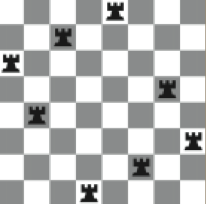
\includegraphics[width=1\textwidth]{img/lhs_chess}
  \end{columns}
\end{frame}


\end{document}
